\section{ANTECEDENTES}
%\section[Antecedentes]{ANTECEDENTES}
A continuación se revisa la evolución de los métodos de visión computacional aplicados en la conducción autónoma y los sistemas resultantes aplicados a esta tarea.
\subsection{ESTADO DEL ARTE}
%\subsection[Estado del Arte]{ESTADO DEL ARTE}
Se revisa el desarrollo de las tecnologías a utilizar desde su creación hasta el momento.

\subsubsection{DETECCIÓN DE OBJETOS}
%\subsubsection[Detección de Objetos]{DETECCIÓN DE OBJETOS}
\paragraph{1963 PERCEPCIÓN DE SÓLIDOS TRIDIMENSIONALES}
Lawrence Roberts desarrollo un algoritmo para detectar figuras sólidas simples en imágenes, extraer su estructura característica en forma de líneas para poder aplicarles transformaciones de perspectiva en un espacio 3D. \citep{Roberts_1963}
% (Robert, 1963)

\begin{figure}[H]
    \centering
    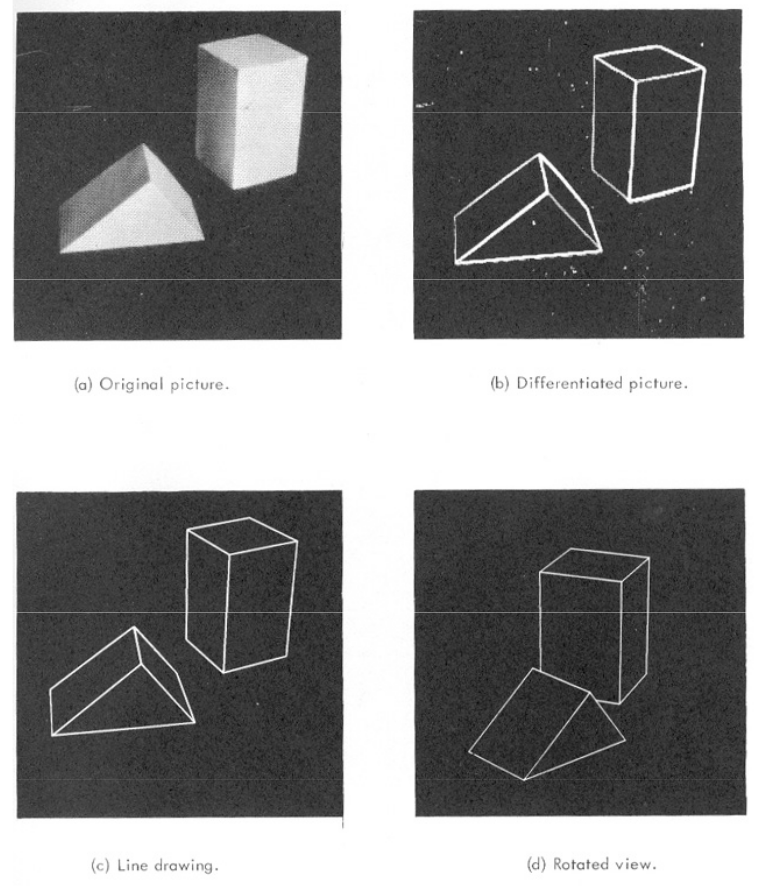
\includegraphics[scale=0.25]{imagenes/machine-perception-of-three-dimensional-solids}
    \caption[Contornos de objetos]{Detección de contornos de objetos\\Fuente: \citep{Roberts_1963}}
\end{figure}
% \vspace{-6mm}
% \begin{center}
%     Fuente: Artículo original
% \end{center}
\paragraph{2001 HAAR FEATURES}
Paul Viola y Michael Jones desarrollaron el algoritmo Viola-Jones, el cual significó un cambio radical en los métodos de detección de objetos, extrayendo características primitivas con clasificadores débiles uno detrás del otro, y aplicando la técnica de la imagen integral, fueron capaces de detectar distintos tipos de objetos en imágenes de manera óptima, entrenando el método sobre un conjunto pequeño de imágenes. Este método se usa hasta hoy en día en cámaras celulares para la detección de rostros. \citep{haar-cascade}
% (Viola \& Jones, 2001)

\begin{figure}[H]
    \centering
    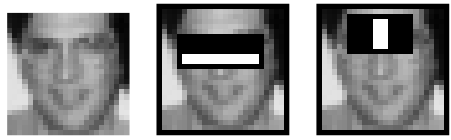
\includegraphics[scale=0.4]{imagenes/haar}
    \caption[Características HAAR]{Características Haar buscando patrones en la imágen\\Fuente: \citep{haar-cascade}}
\end{figure}
% \vspace{-6mm}
% \begin{center}
%     Fuente: Artículo original
% \end{center}
\paragraph{2005 HISTOGRAMAS DE GRADIENTES ORIENTADOS}
En 1986 Robert K. McConnell describe un descriptor de características que sería conocido como HOG o histograma de gradientes orientados, en 2005 sería aplicado a la detección de personas, rivalizando con el método de características Haar. \citep{hog-paper}
% (Dalal \& Triggs, 2005) 

\begin{figure}[H]
    \centering
    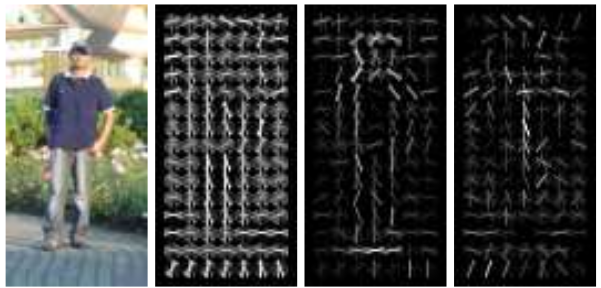
\includegraphics[scale=0.4]{imagenes/hog}
    \caption[Vectores direccionales del HOG]{Vectores direccionales del HOG\\Fuente: \citep{hog-paper}}
\end{figure}
% \vspace{-6mm}
% \begin{center}
%     Fuente: Artículo original
% \end{center}
\paragraph{2016 YOLO}
La búsqueda de métodos que aceleren el proceso de ventanas deslizantes para localizar objetos, llevó a buscar alternativas que realicen todo el proceso en una sola pasada del método, así nace You Only Look Once, una arquitectura de red neuronal convolucional que barre la imágen en grillas definidas buscando la existencia del centro de un objeto y realizando una supresión de no máximo para eliminar ocurrencias repetidas, siendo uno de los métodos más efectivos en la detección de objetos. \citep{Redmon2016YouOL}
% (Redmon, Divvala, Girshick, \& Farhadi)
% \newpage
\begin{figure}[H]
    \centering
    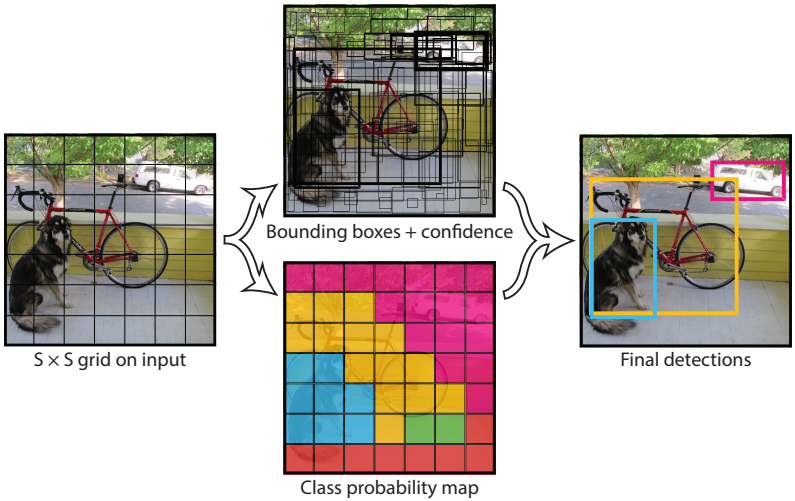
\includegraphics[scale=0.4]{imagenes/yolo}
    \caption[Flujo predicción YOLO]{Flujo predicción YOLO\\Fuente: \citep{Redmon2016YouOL}}
\end{figure}
% \vspace{-6mm}
% \begin{center}
%     Fuente: Artículo original
% \end{center}
\paragraph{2016 SSD}
Con una arquitectura distinta aplicando la misma idea de la partición de la imágen en una grilla, se propone el método Single Shot MultiBox Detector, el cual es menos preciso en la detección de objetos que su contraparte YOLO, pero más rápido y capaz de detectar objetos más pequeños en la imágen. \citep{liu-ssd}
% (Liu et al, 2016)

\begin{figure}[H]
    \centering
    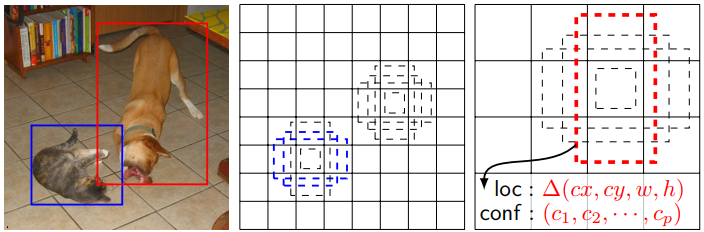
\includegraphics[scale=0.4]{imagenes/ssd}
    \caption[Partición y recuadros de detección SSD]{Partición y recuadros de detección SSD\\Fuente: \citep{liu-ssd}}
\end{figure}
% \vspace{-6mm}
% \begin{center}
%     Fuente: Artículo original
% \end{center}
\paragraph{2020 RETINANET}
Buscando solucionar el problema de la detección de objetos pequeños y en gran cantidad en un entorno denso, mediante modificaciones en la función de costo del clasificador, nace la llamada Retinanet \citep{retinanet}

\subsubsection{SEGMENTACIÓN SEMÁNTICA}
%\subsubsection[Segmentación Semántica]{SEGMENTACIÓN SEMÁNTICA}

\paragraph{SEGMENTACIÓN POR COLOR Y ESCALA DE GRISES}
Entre los primeros métodos de segmentación semántica están los de segmentación por burbujas de color en espacios de color alternativos al RGB, de forma que toda un área de un color específico con alguna variación permitida era enmascarada como un objeto en la imágen.

\paragraph{2004 CAMPOS ALEATORIOS CONDICIONALES MULTIESCALA}
La idea de los campos aleatorios condicionales, (MCRF abreviado en inglés) nació para etiquetar y segmentar secuencias de textos, pero fue modificada para lograr segmentar elementos de una imagen, modelando la relación espacial entre los píxeles con una probabilidad condicional que pertenezca a alguna clase dada la clase de los píxeles vecinos, aplicando un campo estocástico bidimensional (generalización de un proceso estocástico). \citep{segmentation-crf}

\begin{figure}[H]
    \centering
    \subfloat[imágen original]{{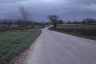
\includegraphics[width=5cm]{imagenes/mcrf1} }}%
    \qquad
    \subfloat[segmentación con MCRF]{{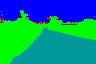
\includegraphics[width=5cm]{imagenes/mcrf2} }}%
    \caption[Segmentación de carretera por MCRF]{Segmentación de carretera por MCRF\\Fuente: \citep{segmentation-crf}}
\end{figure}

\paragraph{2015 U-NET}
Inicialmente pensada para aplicaciones médicas, esta arquitectura de Red Neuronal Convolucional probó ser efectiva en muchas tareas se segmentación, extendiendo la idea de un auto encoder con saltos entre capas, la topología de las conexiones de la red forman una U, de donde proviene su nombre. \citep{u-net}

\begin{figure}[H]
    \centering
    \subfloat[imágen original]{{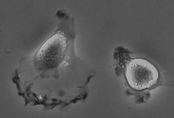
\includegraphics[width=5cm]{imagenes/u-net-1} }}%
    \qquad
    \subfloat[segmentación con U-Net]{{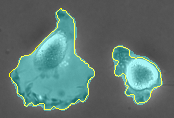
\includegraphics[width=5cm]{imagenes/u-net-2} }}%
    \caption[Segmentación de una célula del dataset PhC-U373]{Segmentación de una célula del dataset PhC-U373\\Fuente: \citep{u-net}}%
    \label{unet}%
\end{figure}
% \vspace{-6mm}
% \begin{center}
%     Fuente: Artículo U-Net
% \end{center}

% \newpage

\paragraph{2017 MASK-RCNN}
Siguiendo la propuesta de una red de dos etapas, dividiendo la tarea en dos más sencillas, esta arquitectura primero propone regiones de interés en base a las cuales hace dos tipos de inferencia, una regresión de los puntos delimitando un rectángulo que encierra a cada objeto, y una máscara binaria para cada clase a segmentar. \citep{mask-rcnn} Junto a la U-Net son los dos métodos más usados en la actualidad, incluido en el dominio de vehículos autónomos.

\begin{figure}[H]
    \centering
    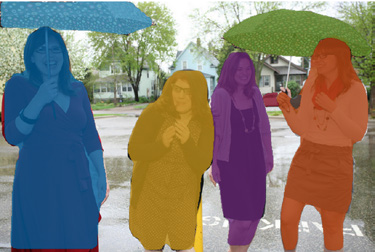
\includegraphics[scale=0.5]{imagenes/maskrcnn}
    \caption[Segmentación semántica de distintas clases]{Segmentación semántica de distintas clases\\Fuente: \citep{mask-rcnn}}
\end{figure}
% \vspace{-6mm}
% \begin{center}
%     Fuente: Artículo original Mask-RCNN
% \end{center}
\subsubsection{SISTEMAS DE CONDUCCIÓN AUTÓNOMA}
%\subsubsection[Sistemas de Conducción Autónoma]{SISTEMAS DE CONDUCCIÓN AUTÓNOMA}

\paragraph{2004 DAVE}
Uno de los primeros intentos de programar un sistema de conducción autónoma fue propuesto por un equipo en el que se encontraba Yann LeCun, uno de los precursores en el uso de las redes convolucionales. En este proyecto se usaban dos cámaras, se entrenó una red en imágenes capturadas en un vehículo a control remoto, y se realizaba una predicción del nivel de aceleración y ángulo de rotación para cada fotograma capturado. \citep{LeCun:04-dave}

\begin{figure}[H]
    \centering
    \subfloat[Vehículo DAVE]{{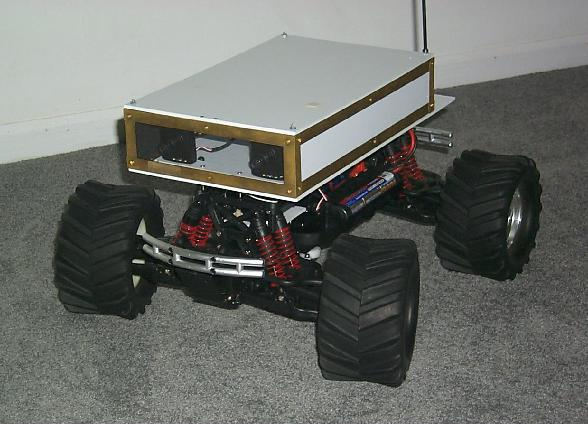
\includegraphics[width=4cm]{imagenes/dave-1} }}%
    \qquad
    \subfloat[Predicción del ángulo de rotación]{{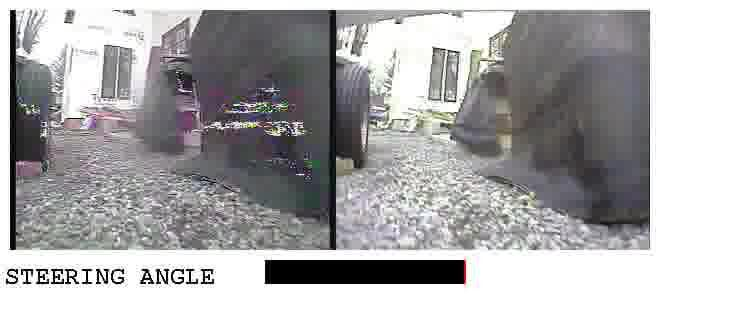
\includegraphics[width=6cm]{imagenes/dave-2} }}%
    \caption[DAVE]{Fuente: Reporte \citep{LeCun:04-dave}}%
    \label{dave}%
\end{figure}

\paragraph{2004 DARPA GRAND CHALLENGE}
La agencia de investigación en proyectos de defensa avanzados o DARPA abreviado en inglés, organizó una comptenecia en el desierto Mojave, con una pista preparada en un terreno arenoso. Los vehículos concursantes podían usar distintos tipos de sensores como cámaras, radar, lidar y GPS. \citep{hooper_2004}

\paragraph{2010 GOOGLE}
Después de muchos tests con asistencia humana y sin llamar la atención, se hacen públicos los experimentos de Google en la vía publica con vehículos equipados con sensores y un sistema de conducción autónoma. Este sistema iría evolucionando hasta la actualidad, cuando después de un cambio de nombre del proyecto, ahora bajo la marca Waymo, Ya realizan trayectos totalmente autónomos. \citep{markoff_2010}

\paragraph{2015 TESLA}
Tesla inició su programa de conducción autónoma oficialmente el año 2015, con un actualización de software para los Tesla Model S equipados con el Hardware necesario para el funcionamiento de su Autopilot. \citep{nelson_2015} Posteriormente después de varias actualizaciones de software, y una de hardware, los distintos vehículos sucesivos de Tesla recopilarían los datos necesarios de los trayectos realizados por los usuarios para mejorar la reacción de este sistema \citep{karpathy-scaledml}

\subsection{TRABAJOS SIMILARES}
%\subsection[Trabajos Similares]{TRABAJOS SIMILARES}

\begin{itemize}[nosep]
    \item[] \textbf{Título:} Aprendizaje fin a fin para la conducción autónoma de vehículos domésticos usando visión artificial y redes neuronales convolucionales.
    \item[] \textbf{Autor:} Jose Eduardo Laruta Espejo
    \item[] \textbf{Año:} 2018
    \item[] \textbf{Institución:} Universidad Mayor de San Andrés
    \item[] Esta tesis plantea implementar un sistema fin a fin embedido, equipado con una raspberry pi, que recibía fotogramas de una pista para carreras y debía predecir con una sola red neuronal, el ángulo de rotación de los servomotores y la aceleración para cada fotograma.
\end{itemize}

\begin{itemize}[nosep]
    \item[] \textbf{Título:} Deep Vision Pipeline for Self-Driving Cars Based on Machine Learning Methods.
    \item[] \textbf{Autor:} Mohammed Nabeel Ahmed
    \item[] \textbf{Año:} 2017
    \item[] \textbf{Institución:} Ryerson University
    \item[] Este trabajo propone un flujo de datos para procesar la información en base a cámaras, mediante detección de las líneas de carreteras, clasificación de signos de tráfico y vehículos para realizar control del vehículo usando la predicción de estos.
\end{itemize}

\begin{itemize}[nosep]
    \item[] \textbf{Título:} Modelamiento Semántico del Entorno para la Conducción Autónoma de un Vehículo Terrestre
    \item[] \textbf{Autor:} Fernando Javier Bernuy Bahamóndez
    \item[] \textbf{Año:} 2017
    \item[] \textbf{Institución:} Universidad de Chile
    \item[] La tesis doctoral, propone el uso de segmentación semántica para apoyar técnicas clásicas de visión computacional para la localización espacial de un vehículo en un entorno urbano, logrando ubicarse en posiciones del terreno, estimar su orientación y lugar del recorrido planeado.
\end{itemize}